\chapter{Multilingual Data and Machine Translation}
\label{ch:mt}

Modern machine translation systems~\citep{koehn-09} use millions of examples of translations to learn translation rules in local (phrase) context, while ignoring the global (document) context. These systems work best when the training corpus has consistent global context, including genre, register, and topic. Systems that are robust to systematic variation in the training set are said to exhibit \textbf{domain adaptation}. 

Topic models are a promising solution for automatically learning semantic coherence and discovering the domain knowledge as global context for applications such as statistical machine translation, including improving the translation models~\citep{Eidelman-12,hu-14,zhao-06,xiao-12,xiong-13} as well as the language coherence~\citep{Bellegarda-04,wood-09}. 
While multiple languages are involved in machine translation, multilingual topic models~\citep{mimno-09,boyd-graber-10} can also be applied to extract better knowledge and apply into machine translation.

\section{Statistical Machine Translation}

Statistical machine translation casts machine translation as a probabilistic process~\citep{koehn-09}. Here we briefly introduce the standard phrase translation model introduced in~\citep{koehn-03}. Given the source sentence $\mathbf{f}$, the best translation in target language $\mathbf{e}_\texttt{best}$ is modeled as,
\begin{equation}
\mathbf{e}_\texttt{best} = \textbf{argmax}_\mathbf{e} p(\mathbf{e}|\mathbf{f}) = \textbf{argmax}_\mathbf{e} p(\mathbf{f}|\mathbf{e}) p (\mathbf{e})
\end{equation}
which is split to a \textit{translation model} $p(\mathbf{f}|\mathbf{e})$ and a \textit{language model} $p (\mathbf{e})$. 

The source sentence $\mathbf{f}$ is segmented into multiple source phrases $\bar{f}_i$ during the decoding, which are translated to a set of target phrases $\bar{e}_i$. Thus the translation probability $p(\mathbf{f}|\mathbf{e})$ can be further decomposed to the phrase translation probability $p(\bar{f}_i | \bar{e}_i)$. Besides, the target phrases may need to be \textit{reordered} to get the best translation result, and this part is captured by a relative distortion probability distribution $d(a_i - b_{i-1})$, where $a_i$ denotes the start position of the source phrase that was translated to the $i$th target phrase, and $b_{i-1}$ denotes the end position of the source phrase translated into the $(i-1)$th target phrase. As a result, the translation model can be decomposed as,
\begin{equation}
p(\mathbf{f}|\mathbf{e}) = \prod_{i} p(\bar{f}_i | \bar{e}_i) d(a_i - b_{i-1})
\end{equation}

In phrase-based \textsc{smt}, the phrase probability $p(\bar{f}_i | \bar{e}_i)$ can be further estimated by combining lexical translation probabilities of words contained in that phrase~\citep{koehn-03}, which is normally referred as \textit{lexical weighting}. Lexical conditional probabilities $p_w(f|e)$ are maximum likelihood estimates from relative lexical frequencies,
\begin{equation}
\label{eq:lexical_prob}
p_w(f|e) = \textstyle \slfrac{c(f, e)}{\sum_f{c(f, e)}}
\end{equation}
where $c(f, e)$ is the count of observing lexical pair $(f, e)$ in the training dataset. Given a word alignment $a$, the lexical weight for this phrase pair $p_w(\bar{f} | \bar{e}; a)$ is the normalized product of lexical probabilities of the aligned word pairs within that phrase pair:
\begin{equation}
\label{eq:phrase_prob}
p_w(\bar{f} | \bar{e}; a) = \prod^{n}_{i=1} \frac{1}{\{|j | (i, j) \in a\}|} \sum_{\forall (i,j) \in a} p_w(f_i | e_j)
\end{equation}
where $i$ and $j$ are the word positions in target phrase $\bar{e}$ and source phrase $\bar{f}$ respectively.

\paragraph{\textsc{smt} with Domain Adaptation}

A \textsc{smt} system is usually trained on documents with the same genre (e.g., sports, business) from a similar style (e.g., newswire, blog-posts).  These are called \emph{domains}.  Translations within one domain are better than translations across domains since they vary dramatically in their word choices and style.  A correct translation in one domain may be inappropriate in another domain.  For example, ``\begin{CJK*}{UTF8}{gbsn}潜水\end{CJK*}'' in a newspaper usually means ``underwater diving''.  On social media, it means a non-contributing ``lurker''.

To Train such \textsc{smt} systems with domain adaptation, early efforts focus on building separate models~\citep{foster-07} and adding features~\citep{matsoukas-09} to model domain information.  \citet{chiang-11} combine these approaches by directly optimizing genre and collection features by computing separate translation tables for each domain.

However, these approaches treat domains as hand-labeled, constant, and known \textit{a priori}.  This setup is at best expensive and at worst infeasible for large data.  Topic models provide a solution where domains can be automatically induced from raw data: treat each topic as a domain. \footnote{Henceforth we will use the term ``topic'' and ``domain'' interchangeably: ``topic'' to refer to the concept in topic models and ``domain'' to refer to \textsc{smt} corpora.}
Such global context from topic models can be applied to improve each component of the statistical machine translation systems. Next we introduce how to apply such domain knowledge from topic models to translation models, language models and reordering models respectively.

\section{Topic Models in Translation Models}

%Topic models have been applied to improve the translation models through domain adaptation~\citep{Eidelman-12,hu-14}, word alignment~\citep{zhao-06} and translation coherence~\citep{xiao-12,xiong-13}.

Topic models are a promising solution for automatically discovering the global context---for example, domain knowledge---in machine translation corpora~\citep{Eidelman-12,hu-14}. Given the soft domain assignments from topic models, \citet{Eidelman-12} extract lexical weighting features conditioned on the topics, optimizing feature weights using the \emph{Margin Infused Relaxed Algorithm}~\citep[\textsc{mira}]{Crammer-06}.

\subsection{Translation Domain Adaptation with Topic Models}

Topic models take the number of topics $K$ and a collection of documents as input, where each document is a bag of words. They output two distributions: a distribution over topics for each document $d$; and a distribution over words for each topic. If each topic defines a \textsc{smt} domain, the document's topic distribution is a soft domain assignment for that document.

Given the soft domain assignments, \citet{Eidelman-12} extract lexical weighting features conditioned on the topics, optimizing feature weights using the \emph{Margin Infused Relaxed Algorithm}~\cite[\textsc{mira}]{Crammer:2006}.  The topics come from source documents \emph{only} and create topic-specific lexical weights from the per-document topic distribution $p(k|d)$, which is used to smooth the expected count $\hat{c}_{k}(f,e)$ of a word translation pair under topic $k$,
\begin{align}
\textstyle \hat{c}_{k}(f,e) = \sum_{d}{p(k|d)c_d(f,e)},
\end{align}
where $c_d(\bullet)$ is the number of occurrences of the word pair in document $d$.  The lexical probability conditioned on topic $k$ is the unsmoothed probability estimate of those expected counts
\begin{align}
\label{eq:lexical_prob_k}
\textstyle p_w(f|e;k) = \hat{c}_{k}(f,e) / \sum_f{\hat{c}_{k}(f,e)},
\end{align}
from which we can compute the lexical weight of this phrase pair
$p_w(\bar{f}|\bar{e};a, k)$ given a word alignment $a$\citep{koehn-03}:
\begin{align}
\label{eq:phrase_prob_k}
p_w(\bar{f} | \bar{e};a, k) = \prod^{n}_{i=1} \frac{1}{\{|j | (i, j) \in a\}|} \sum_{\forall (i,j) \in a} p_w(f_i | e_j; k)
\end{align}
where $i$ and $j$ are the word positions in target phrase $\bar{e}$ and source phrase $\bar{f}$ respectively. Comparing Equation~\ref{eq:lexical_prob_k} against Equation~\ref{eq:lexical_prob}, and Equation~\ref{eq:phrase_prob_k} against Equation~\ref{eq:phrase_prob}, we can clearly see how the topics are encoded as soft domains and how these topics influence the probability. 

For a test document $d$, the document topic distribution $p(k | d)$ is inferred based on the topics learned from training data. The lexical weight feature of a phrase pair $(\bar{f}, \bar{e})$ is,
\begin{align}
\textstyle f_{k}(\bar{f}|\bar{e})=-\log\left\{{p_{w}(\bar{f}|\bar{e};k)\cdot p(k|d)}\right\},
\end{align}
a combination of the topic dependent lexical weight and the topic distribution of the document, from which we extract the phrase.

In fact, \citet{Eidelman-12} introduces the two direction topic-adapted probabilities instead of a single direction: $p_w(\bar{f} | \bar{e};a, k)$ and $p_w(\bar{e} | \bar{f};a, k)$. This is equivalent to introduce $2K$ new word translation tables, thus it results in introducing $2K$ lexical weight features $f_{k}(\bar{f}|\bar{e})$ and $f_{k}(\bar{e}|\bar{f})$. Given the topic-adapted features, \citet{Eidelman-12} compute the resulting model score by combining these adapted features in a linear model with other standard \textsc{smt} features and optimizing the weights:
\begin{align}
\explain{standard features}{\sum_p \lambda_p f_p(\bar{f},\bar{e})} + \explain{adapted features}{\sum_k \lambda_k f_k(\bar{f} | \bar{e})} + \explain{adapted features}{\sum_k \lambda_k f_k(\bar{e} | \bar{f})}
\end{align}
These adapted features allow us to bias the translations according to the topics. For example, if topic $k$ is dominant in a test document, the feature $f_k(\bar{f} | \bar{e})$ will be large, which may bias the decoder to a translation that has small value of the standard feature $f_p(\bar{f}, \bar{e})$. In addition, combining the adapted features with the standard features makes this model more flexible. For a test document with less clear topics, the topic distribution will tend toward being fairly uniform. In this case, the topic features will contribute less to the translation results and the standard features will dominate the translation results.

Conceptually, this approach is just reweighting examples.  The probability of a topic given a document is never zero.  Every translation observed in the training set will contribute to $p_{k}(e|f)$; many of the expected counts, however, will be less than one.  This obviates the explicit smoothing used in other domain adaptation systems~\citep{chiang-11}.

\citet{su-12} introduce the topics to machine translation based on a similar idea but using \emph{hidden topic Markov models}~\citep[\textsc{htmm}]{gruber-07} to monolingual data. They incorporate the topic information from the source language into translation probability estimation, and decompose the phrase probability $p(\bar{e}|\bar{f})$ as,
\begin{align}
p(\bar{e}|\bar{f}) = \sum_{t_f} p(\bar{e}, t_f | \bar{f}) = \sum_{t_f} p(\bar{e} | \bar{f}, t_f) \cdot p(t_f | \bar{f})
\end{align}
where $p(\bar{e} | \bar{f}, t_f)$ is the translation probability given the source side topic $t_f$, and $p(t_f | \bar{f})$ denotes the phrase probability in topic $t_f$. \textsc{htmm} is applied to the out-of-domain source data to estimate the topic $t_f$ and further estimate $p(\bar{e} | \bar{f}, t_f)$ as $p(\bar{e} | \bar{f}, t_{f_out})$, and \textsc{htmm} is also applied to the in-domain source data to compute $p(t_f | \bar{f})$ as $p(t_{f_in} | \bar{f})$. However, $t_{f_out}$ and $t_{f_in}$ may not be in the same space, so \citet{su-12} introduce the topic mapping probability $p(t_{f_out} | t_{f_in})$ to map the in-domain topic to the out-of-domain topic:
\begin{align}
p(t_{f_out} | \bar{f}) = \sum_{t_{f_in}} p(t_{f_out} | t_{f_in}) \cdot \cdot p(t_{f_in} | \bar{f})
\end{align}
Thus the final phrase probability can be refined as,
\begin{align}
p(\bar{e}|\bar{f}) = \sum_{t_{f_out}} \sum_{t_{f_in}} p(\bar{e} | \bar{f}, t_{f_out}) \cdot p(t_{f_out} | t_{f_in}) \cdot p(t_{f_in} | \bar{f})
\end{align}

\citet{hasler-12} also apply \textsc{htmm} and introduce sparse word pair features and phrase pair features based on topic models for domain adaptation to improve the \textsc{smt} system. They apply \textsc{htmm} on the source documents, and assign one topic to the whole sentence. Then the topic information is integrated as a source side trigger for a particular word pair or phrase pair, given a topic. For  example, given a sentence pair $(s_f, s_e)$ with topic $k$, for an aligned word pair $(w_f, w_e)$ which is observed $c$ times in this sentence pair, the sparse word pair feature $wp$ with topics is represented as $wp\_k\_w_f \sim w_e = c$, while the original word pair feature is $wp\_w_f \sim w_e = c$. Similarly, the topic phrase pair features are also defined: given an aligned phrase pair $(p_f, p_e)$ with count $c$ in the same sentence, the sparse phrase pair feature $pp$ with topics is represented as $pp\_k\_p_f \sim p_e = c$. Both the phrase pair and word pair features are extracted from the aligned training sentence pairs, and then the Margin Infused Relaxed Algorithm~(MIRA)~\citep{Crammer-06} are used to learn the feature weights. The evaluation on both English-French and German-English shows promising results.

However, \citet{Eidelman-12,su-12,hasler-12} ignore a wealth of information that could improve topic models and help machine translation. They rely solely on monolingual source-side models. In contrast, machine translation uses inherently multilingual data: an \textsc{smt} system must translate a phrase or sentence from a \emph{source} language to a different \emph{target} language, so existing applications of topic models~\citep{Eidelman-12,su-12,hasler-12} are ignoring available information on the target side that could aid domain discovery. This can be improved by introduction multilingual topic models for machine translation, and the details are introduced in the next section.

\subsection{Multilingual Information for Domain Adaptation}
\label{sec:trans-multiling}

As we mentioned in the previous section, \citet{Eidelman-12,su-12,hasler-12} only use monolingual data from the source language for topic modeling, ignoring all target-language data and available lexical semantic resources between source and target languages. In fact, different languages complement each other to reduce ambiguity.  For example, ``\begin{CJK*}{UTF8}{gbsn}木马\end{CJK*}'' in a Chinese document can be either ``hobbyhorse'' in a children's topic, or ``Trojan virus'' in a technology topic.  A short Chinese context obscures the true topic. However, these terms are unambiguous in English, revealing the true topic. From this example, we can see that that topic models on multilingual corpus do improve the quality of the extracted topics.

There are various ways to build up the multilingual topic models. Different languages can be connected on the word-level or the document levels. 
On one hand, \emph{lexical information}, such as orthographic similarity~\citep{boyd-graber-09} and multilingual dictionaries~\citep{boyd-graber-10}, can be very helpful to induce better topics from multilingual corpora. For instance, tree-based topic models~\citep{boyd-graber-07,andrzejewski-09,Hu:Boyd-Graber:Satinoff-ur} incorporate the correlations between words in the same or different languages by encouraging words that appear together in a {\bf concept} to have similar probabilities given a topic. 
On the other hand, topic models can take advantage of document \emph{alignment information} and infer more robust topics from the aligned dataset. For example, polylingual topic models~\citep{mimno-09} assume that the aligned documents in different languages share the same topic distribution and each language has a unique topic distribution over its word types. 

These two approaches are not mutually exclusive, however; they reveal different connections across languages. \citet{hu-14} bring existing tree-based topic models~(\tlda{}) and polylingual topic models~(\plda{}) together and create the polylingual tree-based topic model~(\ptlda{}) that incorporates both word-level correlations and document-level alignment information. They further apply the proposed polylingual tree-based topic model in the \textsc{smt} framework from \citet{Eidelman-12} to improve the machine translation results.

\paragraph{\bf Word-level Correlations}

Tree-based topic models incorporate the positive correlations between words by encouraging words that appear together in a {\bf concept}~(referred as ``positive correlations'' in \citet{andrzejewski-09,Hu:Boyd-Graber:Satinoff-ur}) to have similar probabilities given a topic. These concepts can come from WordNet~\citep{boyd-graber-10}, domain experts~\citep{andrzejewski-09}, or user constrains~\citep{Hu:Boyd-Graber:Satinoff-ur}. When we gather concepts from bilingual resources, these concepts can connect different languages.  For example, if a bilingual dictionary defines ``\begin{CJK*}{UTF8}{gbsn}电脑\end{CJK*}'' as ``computer'', we combine these words in a concept.

These concepts (positive correlations) are organized into a {\bf prior tree} structure. As Figure~\ref{fig:prior_trees} shows, words in the same concept share a common parent node, and then that concept becomes one of many children of the root node.  Words that are not in any concept---{\bf uncorrelated words}---are directly connected to the root node.

When this tree serves as a prior for topic models, words in the same concept are positively correlated in topics. 
For example, if ``\begin{CJK*}{UTF8}{gbsn}电脑\end{CJK*}'' has high probability in a topic, so will ``computer'', since they share the same parent node. With the tree priors, each topic is no longer a distribution over word types; instead, it is a distribution over paths, and each path is
associated with a word type.  The same word could appear in multiple paths, and each path represents a unique sense of this word.

\paragraph{\bf Document-level Alignments}

Lexical resources connect languages and help guide the topics. However, these resources are sometimes brittle and may not cover the whole vocabulary.  Aligned document pairs provide a more corpus-specific, flexible association across languages.

\citet{Landauer-1990} connect documents in different languages by projecting both documents to a shared latent semantic indexing space. Similarly, 
polylingual topic models~\citep{mimno-09} assume that the aligned documents in different languages share the same topic distribution and each language has a unique topic distribution over its word types.  This connection between languages is flexible: instead of requiring the exact matching on words and sentences, only a coarse document alignment is necessary, as long as the documents discuss the same topics.

\paragraph{\bf Combine Words and Documents}

\citet{hu-14} introduce polylingual tree-based topic models (\ptlda{}), which connect information across different languages by incorporating both
word correlation (as in \tlda{}) and document alignment information (as in \plda{}). 

To build up the prior tree structure, \citet{hu-14} consider two resources to build trees that correlate words across languages. The first is multilingual dictionaries~(\textit{dict}), which match words with the same meaning in different languages together.  These relations between words are used as the concepts~\citep{Bhattacharya-2006} in the prior tree.% (Figure~\ref{fig:prior_trees}). 
In addition, they extract the word alignments from aligned sentences in a parallel corpus.  The word pairs define concepts for the prior tree (\textit{align}). 

%\begin{figure}
%\centering
%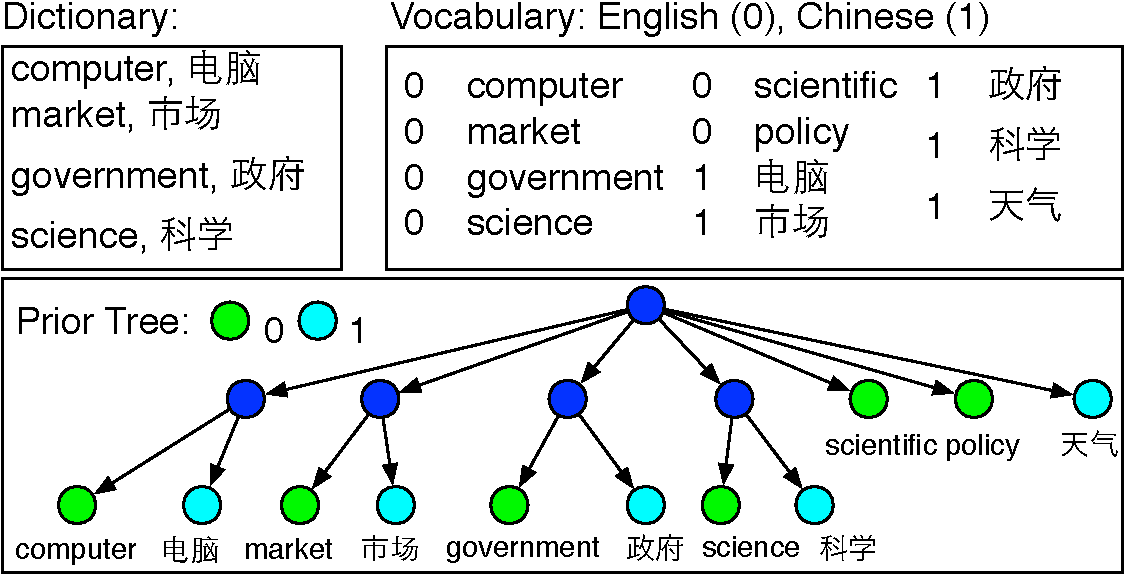
\includegraphics[width=0.9\linewidth]{figures/correlations_tree-crop.pdf}
%\vspace{-3mm}
%\caption[Constructing prior tree from a bilingual dictionary]{An example of constructing a prior tree from a
%  bilingual dictionary: word pairs with the same meaning but in
%  different languages are concepts; we create a common parent node to
%  group words in a concept, and then connect to the root;
%  uncorrelated words are connected to the root directly.  Each topic
%  uses this tree structure as a prior. }
%\label{fig:prior_trees}
%\end{figure}

Given the prior tree structure, the proposed polylingual tree-based topic models introduce an additional step of selecting a concept in a topic responsible for generating each word token. This is represented by a path $y_{d,n}$ through the topic's tree. This is the same as \tlda{}, but different from \abr{lda}, where each word is associated with a topic. 

%\begin{algorithm}[t!]
%\begin{footnotesize}
%\caption{\textsc{\small{Generative Process for \ptlda{}}}}
%\label{alg:ptlda}
%\begin{algorithmic}[1]
%  \FOR{topic $k \in {1, \cdots, K}$}
%  \FOR{each internal node $n_i$}
%  \STATE draw a distribution $\pi_{ki} \sim \text{Dir}(\beta_i)$
%  \ENDFOR
%  \ENDFOR
%  \FOR{document set $d \in {1, \cdots, D}$}
%  \STATE draw a distribution $\theta_d \sim \text{Dir}(\alpha)$
%  \FOR{each word in documents $d$}
%  \STATE choose a topic $z_{dn} \sim \text{Mult}(\theta_d)$
%  \STATE sample a path $y_{dn}$ with probability $\prod_{(i,j) \in y_{dn}} \pi_{z_{dn}, i, j}$
%  \STATE $y_{dn}$ leads to word $w_{dn}$ in language $l_{dn}$
%  \STATE append token $w_{dn}$ to document $d_{l_{dn}}$
%  \ENDFOR
%  \ENDFOR
%\end{algorithmic}
%\end{footnotesize}
%\end{algorithm}


The probability of a path in a topic depends on the transition probabilities in a topic.  Each concept $i$ in topic $k$ has a distribution over its children nodes is governed by a Dirichlet prior: $\pi_{k,i} \sim \text{Dir}(\beta_{i})$.  Each path ends in a word (i.e., a leaf node) and the probability of a path is the product of all of the transitions between topics it traverses. Topics have correlations over words because the Dirichlet parameters can encode positive or negative correlations~\citep{andrzejewski-09}.

With these correlated in topics in hand, the generation of documents is very similar to \textsc{lda}.  For every document $d$, we first sample a distribution over topics $\theta_d$ from a Dirichlet prior $\text{Dir}(\alpha)$.  For every token in the documents, we first sample a topic $z_{dn}$ from the multinomial distribution $\theta_d$, and then sample a path $y_{dn}$ along the tree according to the transition distributions specified by topic $z_{dn}$.  Because every path $y_{dn}$ leads to a word $w_{dn}$ in language $l_{dn}$, we append the sampled word $w_{dn}$ to document $d_{l_{dn}}$.  Aligned documents have words in both languages; monolingual documents only have words in a single language. 
%The full generative process is shown in Algorithm~\ref{alg:ptlda}.

If a flat symmetric Dirichlet prior is used instead of the tree prior, \plda{} is recovered; and if all documents are monolingual (i.e., with distinct distributions over topics $\theta$), \tlda{} is recovered. \ptlda{} connects different languages on both the word level (using the word correlations) and the document level (using the document alignments).

While \citet{hu-14} incorporate the topic information at the phrase level, \citet{xiao-12} propose to incorporate the topic information directly at the rule level rather than the word level. They associate each synchronous rule and each document with a topic distribution, and then select the best rule by comparing their topic similarity. Though monolingual topic models are applied on the source language and target language respectively, they learn the projection between the topics on the target side and the topics on the source side.

More specifically, they build up a monolingual topic model on the source documents and target documents respectively to learn the document-topic distribution $p(z|d)$. Take the source language as an example. If a rule $r$ is used in document $d$ with a topic distribution $p(z|d)$, they collect the instance $I=(r, p(z|d), c)$, where $c$ is the instance fraction count. From the instances $\mathcal{I}$, the rule-topic distribution $p(z=k|r)$ can be computed as,
\begin{align}
p(z=k|r) = \frac{\sum_{I \in \mathcal{I}} c \times p(z=k|d)}{\sum_k \sum_{I \in \mathcal{I}} c \times p(z=k'|d)}
\end{align}

Both the rule-topic distribution on the source side $p(z_f|r)$ and the rule-topic distribution on the target side $p(z_e|r)$ are computed. However, during the decoding, only the document-topic distribution on the source side is available. In order to compute the topic similarity, the rule-topic distribution on the target side should be mapped to the source side. The topics on both the source side and target side are estimated respectively,  and each sentence pair is denoted as $z_f, z_e, a$, where $a$ is the alignment between the source sentence and target sentence as a set of links $\{(i,j)\}$. Then the occurrence of a source-side topic w$k_f$ and a target-side topic $k_e$ is calculated as,
\begin{align}
\sum_{(z_f,z_e,a)} \sum_{(i,j) \in a} \delta(z_{f_i}, k_f) \delta(z_{e_j}, k_e)
\end{align}
where $\delta_{x,y}$ is $1$ if $x=y$ and $0$ otherwise. Then the projection probability $p(z=k_f | z=k_e)$ is computed by normalizing the co-occurrence count. The whole mapping matrix is denoted as $M_{k_e \times k_f}$, and each entry $M_{i,j}$ is $p(z_e=i | z_f=j)$. Then the target-side rule-topic distribution $p(z_e|r)$ can be projected to the source topic space by,
\begin{align}
T(p(z_e|r)) = p(z_e|r) \bigotimes M_{k_e \times k_f}
\end{align}

Given the rule-topic distribution and the document-topic distribution, the topic similarity can be computed as,
\begin{align}
\texttt{Similarity}(p(z|d), p(z|r)) = \sum_{k=1}^{K} (\sqrt{p(z=k|d)} - \sqrt{p(z=k|r)})^2
\end{align}

Two similarity scores are considered as features during decoding: $\texttt{Similarity}(p(z_f|d), p(z_f|r))$, $\texttt{Similarity}(p(z_f|d), T(p(z_e|r)))$. To better distinguish the general-domain data from the in domain data, \citet{xiao-12} also divide the rules into topic-insensitive rules and topic-sensitive rules based on their rule-topic distribution. However, \citet{xiao-12} further notice that some rules are not sensitive to topics, and the topic-insensitive rules should be preferred more than the topic-sensitive rules in this case. To address this issue, they further define the topic sensitivity of a rule:
\begin{align}
\texttt{Sensitivity}(p(z|r)) = - \sum_{k=1}^{K} p(z=k|r) \times \log(p(z=k|r))
\end{align}

As a result, two more sensitivity features are also introduced in the decoding process: $\texttt{Sensitivity}(p(z_f|r))$ and $\texttt{Sensitivity}(p(z_e|r))$. Through introducing the four new features, \citet{xiao-12} significantly improve the translation performance on NIST Chinese-to-English translation experiments.

\section{Topic Models in Language Modeling}

Topic models capture document-level properties of language, but a critical component of machine translation systems is the language model, which provides local constraints and preferences. Domain adaptation for language models~\citep{Bellegarda-04,wood-09} is an important avenue for improving machine translation, as \citet{Bellegarda-04} points out that `` an adaptive language model seeks to maintain an adequate representation of the current task domain under changing conditions involving potential variations in vocabulary, syntax, content, and style''.

A language model describes the probability of a word $w$ occurring given the previous context words, which is also mentioned as the history $h$. Language model adaptation uses extra knowledge to adjust this probability $p(w|h)$ to reflect the content change. Topics from topic models can be one of the resources to provide such knowledge for language model adaptation.

\subsection{Monolingual Topic Models for Language Model Adaptation}

Early work such as \citet{Clarkson-1997,Seymore-1997,Kneser-1997,Iyer-1999} focus on partitioning the training data to multiple topic-specific subsets and building up language models for each subset. Then the topic-specific language models $p_k(w|h)$ are linearly combined with a general language model $p_g(w|h)$ built from all training data as Equation~\ref{eq:linear_lm}. The weights $\lambda_k$ can be tuned based on the topics of the test documents. 
\begin{align}
\label{eq:linear_lm}
p_\textrm{adapted}(w|h) = \sum_k \lambda_k p_k(w|h) + \lambda_g p_g(w|h)
\end{align} 

\citet{Seymore-1998} further identify the most qualified topic for each word in the vocabulary and choose a topic-specific language model or the general language model. The intuition is that the general language model provides the most reliable estimation for general words, and the topic language model estimates the probability more accurately for topic words. As a result, they split the vocabulary words into three groups: the general subset, on-topic subset and off-topic subsets. For general subset and off-topic subset, the general language model provides the word probability; and the topic-specific language model provides the word probability for the on-topic subset. 

While these early attempts introduce the topic mixture to improve the language models, these topic-specific language models are just like the traditional n-gram models, which can model the limited history. Besides, these models assume each document or history belongs to exactly one topic cluster. 

To fix these problems, \citet{Bellegarda-1997,Coccaro-1998} introduce the \emph{Latent Semantic Analysis}~\citep[\textsc{lsa}]{deerwester-90} to learn large-span language model. However, \textsc{lsa} is based on Singular Value Decomposition techniques. Thus \citet{Gildea-1999} further introduces the probabilistic interpretation---the probabilistic latent semantic indexing~\citep[\textsc{plsi}]{hoffman-99}---to language models. \citet{Gildea-1999} decomposes the language model based on topics,
\begin{align}
\label{eq:plsi_lm}
p(w|h) = \sum_k p(w|k) p(k|h)
\end{align}
where the topics are learned from the training corpus by optimizing the log probability,
\begin{align}
l(\theta; N) = \sum_w \sum_d n(w,d) \log \sum_k p(w|k) p(k|d)
\end{align}
where $d$ is the training documents, and $n(w,d)$ is the word frequency of $w$ in document $d$. $p(w|k)$ and $p(k|d)$ are learned through the EM algorithm. For test documents, they fix $p(w|k)$ to estimate $p(t|h)$ and then compute $p(w|h)$ using Equation~\ref{eq:plsi_lm}. However, the topic models do not take advantage of short-range structure. To combine the topic models with the general n-gram language model, \citet{Gildea-1999} assume that the history $h$ and the n-gram context are independent conditioned on $w_i$ as the following,
\begin{align}
p(w_i|h,w_{i-n+1}^{i-1}) \approx \frac{p(w|h)p(w|w_{i-n+1}^{i-1})}{p(w_i)}
\end{align}
Even though this assumption is not valid in general, it works better than the linear scale or log-scale combination according to \citet{Gildea-1999}.

\subsection{Multilingual Topic Models for Language Model Adaptation}

So far the topic models for language model adaptation we have introduced focus on monolingual language. As we explained in Section~\ref{sec:trans-multiling}, the information from different languages can complement each other to extract better topics. In order to introduce multilingual information to topic models, various approaches such as \cite{Tam-2007}, \cite{Ruiz-2011}, \cite{Yu-2013} etc., have been explored. More details are introduced in this section.
%\cite{Tam-2007} introduces the bilingual latent semantic analysis to enforce such one-to-one topic correspondence between the source language and the target language; \cite{Ruiz-2011} merges the aligned the source document and target document together to extract topics; \cite{Yu-2013} builds up topic models from the source language and target language respectively, and then learn the projection relations between source topics and target topics. More details 

\cite{Tam-2007} introduces the bilingual latent semantic analysis~(\textsc{blsa}) to learn the topics for both source language and target language and applies the learned topics into language model adaptation for statistical machine translation. \textsc{blsa} is to transfer the inferred topics from the source language to the parallel target language. In order to enforce such one-to-one topic correspondence between source language and target language, \cite{Tam-2007} introduces the Latent Dirichlet Tree Allocation~(\textsc{ldta}), where the correlation among latent topics are captured using a Dirichlet-Tree prior. The basic idea is that each aligned topic pair are sampled from the same Dirichlet distribution.

More specifically, \cite{Tam-2007} assume the aligned source document and the target document share the same document-topic distribution, thus they first learn a \textsc{lsa} model on the source language. Then they use this document-topic distribution from the source document as the document-topic distribution for the aligned target document, and then infer the topic-word distribution on the target side. The topics on the target language are not learned iteratively, thus the topics in parallel corpus can be learned very efficiently. Then the word marginal distributions are computed and integrated into the target background language model using marginal adaptation~\citep{Kneser-1997b}, which minimizes the KL divergence between the adapted language model and the background language model:
\begin{align}
\label{eq:mdi}
p_a(w|h) \propto \Big( \frac{p_{lsa}(w)}{p_{bg}(w)} \Big) ^{\beta} \cdot p_{bg}(w|h)
\end{align}

\cite{Ruiz-2011} proposes a simplified bilingual topic modeling for language model adaptation. Based on the assumption that the aligned source document and target document share the same document-topic distribution, they combine the aligned source document and target document as one single document and perform the probabilistic latent semantic analysis, from which the conditional probability $p(w|d)$ is computed as:
\begin{align}
p(w|d) = \sum_k p(w|k) p(k|d)
\end{align}
Then the word-document probabilities are converted into pseudo counts via the following scaling function:
\begin{align}
n(w|d) = \frac{p(w|d)}{\max_{w'} p(w'|d)} \cdot \Delta
\end{align}
where $\Delta$ is a scaling factor to raise the probability ratios above 1. They then focus only on the words in target language model and build up a topic-adapted language model. They further combine their new language model with the background language model following Minimum Discrimination Information~(\textsc{MDI}) estimation~\cite{Kneser-1997b} as Equation~\ref{eq:mdi}. 

\citet{Yu-2013} introduces the hidden topic markov model to improve the language model in \textsc{smt}. They build up a topic model on the source side and target side respectively, and learn a topic-specific language model based on the target side by estimating the maximum-likelihood. To smooth the sharply distributed probabilities, back-off probabilities are also considered as follows:
\begin{align}
p(w_i | w^{i-1}_{i-n+1}, k_e) = &\lambda_{w^{i-1}_{i-n+1}} p_{MLE}(w_i|w^{i-1}_{i-n+1}, k_e) \\
&+ (1- \lambda_{w^{i-1}_{i-n+1}})p(w_i|w^{i-1}_{i-n+2}, k_e)
\end{align}
where $\lambda$ is the normalization parameter, calculated by,
\begin{align}
\lambda_{w^{i-1}_{i-n+1}, k_e} = \frac{N_{1+}(w^{i-1}_{i-n-1}, k_e)}{N_{1+}(w^{i-1}_{i-n-1}, k_e) + \sum_{w_i}c(w^i_{i-n+1}, k_e)}
\end{align}
where $N_{1+}(w^{i-1}_{i-n-1}, k_e)$ is the number of words following $w^{i-1}_{i-n-1}$ in topic $k_e$, and $c(w^i_{i-n+1}, k_e)$ is the count of n-gram $w^i_{i-n+1}$ in $k_e$.

During the decoding, since no target sentence is available, they use the topic model on the source side to predict the topics for the testing data, and then project the source topic to the target topic, and then estimate the probability as following:
\begin{align}
p(e) = \sum_{k_e} p(e|k_e) p(k_e) = \sum_{k_e} p(e|k_e) \cdot \sum_{k_f} p(k_e|k_f) p (k_f)
\end{align}
where $p(k_e|k_f)$ is the topic projection probability, estimated by the co-occurrence of the source-side and the target-side topic assignment.

\section{Reordering with Topic Models}

In addition to translation models and languages models, topic models have also been applied to improve the reordering model, another important component in statistical machine translation.

A lexicalized reordering model is to learn the orientation probabilities for a given phrase pair with respect to the previous phrase pair and the following phrase pair~\citep{Chen-2013}. The orientation $o$ typically includes three types: monotone (M), swap (S) and discontinuous (D). The M orientation means the current phrase pair is immediately to the right of the previously translated phrase in the source sentence, S orientation occurs when the current phrase is immediately to the left of the previous phrase, and all other cases all belong to D orientation. This type of reordering model is normally referred as lexicalized since the estimated orientations depend on the words in both the previously translated phrase pair and the current phrase pair. Formally, the reordering model is defined to estimate the corresponding probabilities $p(o|f,e)$ using recursive MAP smoothing:
\begin{align}
p(o|f,e) &= \frac{c(o,f,e) + \alpha_f p(o|f) + \alpha_e p(o|e)}{c(f,e) + \alpha_f + \alpha_e} \\
p(o|f) &= \frac{c(o,f) + \alpha_g p(o)}{c(f) + \alpha_g} \\
p(o|e) &= \frac{c(o,e) + \alpha_g p(e)}{c(e) + \alpha_g} \\
p(o) &= \frac{c(o) + \alpha_u/3}{c(\cdot) + \alpha_u}
\end{align}
where $c(o,f,e)$ is the orientation counts obtained from the word-aligned corpus;  the parameters $\alpha_f$, $\alpha_e$, $\alpha_g$ and $\alpha_u$ are learned by minimizing the perplexity of the resulting model on the held-out data.

\citet{Chen-2013} find that training corpus in different domains vary significantly in their reordering characteristics for particular phrase pairs, thus they introduce the linear model for reordering model adaptation. Given $N$ sub-corpora (or $N$ domain corpus), they first train a reordering model on each domain corpus, and then define the global reordering model as a linear combination of the reordering models on each domain corpus:
\begin{align}
p(o|f,e) = \sum_{i=1}^{N} \alpha_i p_i(o|f,e)
\end{align}
where $p_i(o|f,e)$ is the reordering model on sub-corpus $i$, and the weight $\alpha_i$ are learned by maximizing the probability of phrase-pair orientations in the in-domain development set:
\begin{align}
\hat{\alpha} = \texttt{argmax}_{\alpha} \sum_{o,f,e} \tilde{p}(o,f,e) \log \sum_{i=1}^N \alpha_i p_i(o|f,e)
\end{align}
where $\tilde{p}(o,f,e)$, proportional to $c(o,f,e)$, is the empirical distribution of counts in the development set. \citet{Chen-2013} propose to smooth the in-domain sample and weight instances by document frequency to further improve the mixture adaptation. They demonstrate this adaptation significantly improve the statistical machine translation system.

However, \citet{Chen-2013} manually divide the training data into multiple domains, instead of using automatic techniques such as topic models. \citet{wang-14} introduce topic models to the maximum entropy based phrase reordering models, proposed by \citet{Xiong-2006}. Under the ITG constraints~\citep{Wu-1997}, three Bracketing Transduction Grammar (BTG) rules are used to constrain the translation and reordering:
\begin{align}
A &\rightarrow [A^1, A^2]\\
A &\rightarrow <A^1, A^2>\\
A &\rightarrow f/e
\end{align}
where $A$ is a block with a pair of source and target strings; $A^1$ and $A^2$ are two consecutive blocks; the two rules are reordering rules which merge two blocks into a larger block in a straight or inverted order. Rule 3 translates a source phrase $f$ to a target phrase $e$ and generate a block $A$. These three rules are continuously used until the whole source sentence is covered, and a hierarchical segmentation tree of the source sentence is generated at the same time. Based on this hierarchical setting, \citet{Xiong-2006} treat the reordering problem as a classification with two labels: straight and inverted between two consecutive blocks, and build up a maximum entropy classification model as the reordering model:
\begin{align}
p(o|C(A^1, A^2)) = \frac{\exp(\sum_i \theta_i f_i(o, c(A^1, A^2)))}{\sum_{o'} \exp(\sum_i \theta_i f_i(o', c(A^1, A^2)))}
\end{align}
where $\theta_i$ are the feature weights, $C(A^1, A^2)$ indicates the attributes of $A^1$ and $A^2$, and $f_i(o, C(A^1, A^2))$ are binary features defined as, 
\begin{align}
f_i(o, C(A^1,A^2)) = \begin{cases}
1, &\text{if $(o,C(A^1, A^2)$ satisfies certain condition} \\
0, &\text{else}
\end{cases}
\end{align}

Different from the lexicalized reordering model, this framework only uses the features extracted from the blocks instead of the whole block, thus it is flexible to reorder any blocks~\citep{Xiong-2006}. Following this framework, \citet{wang-14} integrate two more types of topic-based features into the reordering model, in additional to the boundary word features used in \citet{Xiong-2006}. First, they choose the topic with maximum probability in a document to be the \textit{document topic feature} for that document. Besides, they also use the topics of the content words that locate at the left and rightmost positions on the source phrases as the \textit{word topic features} to capture topic-sensitive reordering patterns. During the decoding process, \citet{Xiong-2006} infer the topic distributions of the test documents first and then apply this proposed topic-based reordering model as one sub-model to the log-linear model to obtain the best translation:
\begin{align}
e_\texttt{best} = \texttt{argmax}_e \Big \{ \sum_{m=1}^M \lambda_m h_m(e,f) \Big \}
\end{align}
where $h_m(e,f)$ are the  sub-models or features of the whole log-linear model, $\lambda_m$ are their weights accordingly, which are tuned on the development set.

\section{Beyond Domain Adaptation}

\subsection{Word Alignment with Topic Models}

In addition to applying topic models as domain adaptation, \citet{zhao-06} build up a novel bilingual topical admixture (BiTAM) to improve the word alignment in statistical machine translation. 

BiTAM captures the latent topical structure and generalizes word alignments and translations via topics shared across sentence pairs:
\begin{align}
\textbf{E}^{*} = \texttt{argmax}_{\{\textbf{E}\}} p(\textbf{F} | \textbf{E})p(\textbf{E})
\end{align}
where $p(\textbf{F} | \textbf{E})$ is a document-level translation model, generating the document $\textbf{F}$ as one entity. BiTam assumes each document pair $(\textbf{F}, \textbf{E})$ is an admixture of topics, thus the topics for each sentence pair within that document pair are sampled from the same document-topic distribution $\theta$. Therefore, the sentence-level word alignment and translations are coupled by the hidden topics.  Based on this assumption, \citet{zhao-06} develop three BiTAM models.

Given the document topic mixture $\theta_d$, the first BiTAM model assumes each sentence pair has a single topic $k$, and each topic has a topic-specific translation table $B_k$, where $B_{i,j,k} = p(f_j | e_i, z=k)$. The generative process for a document pair $(\textbf{F}_d | \textbf{E}_d)$ is as follows:
\begin{enumerate}
\item Sample sentence number $N \sim \texttt{Poisson}(\gamma)$.
\item Sample document-topic distribution $\theta_d \sim \texttt{Dirichlet}(\alpha)$.
\item For each sentence pair $(f_n, e_n)$ in the document pair:
\begin{enumerate}
\item Sample sentence length $J_n \sim \texttt{Poisson}(\delta)$.
\item Sample a topic $z_{dn} \sim \texttt{Multinomial}(\theta_d)$.
\item Sample $e_j \sim p(e_j)$, where $p(e_j)$ is a monolingual model.
\item Sample each word alignment link $a_j \sim p(a_j)$, $p(a_j)$ is a uniform model.
\item Sample each $f_j \sim p(f_j | \textbf{e}, a_j, z_n, \textbf{B})$.
\end{enumerate}
\end{enumerate}

Given the model parameters $\alpha$ and $\textbf{B}$, the joint conditional distribution can be written as,
\begin{align}
p(\textbf{F}, \textbf{A}, \theta, \textbf{z} | \textbf{E}, \alpha, \textbf{B}) = p(\theta | \alpha) \prod_{n=1}^{N}p(z_n | \theta)p(\textbf{f}_n, \textbf{a}_n | \textbf{e}_n, \alpha, B_{z_n})
\end{align}
Marginalizing out $\theta$ and $z$, the marginal conditional probability is:
\begin{align}
p(\textbf{F}, \textbf{A} | \textbf{E}, \alpha, \textbf{B}) = \int p(\theta | \alpha) \Big ( \prod_{n=1}^{N} \sum_{z_n} p(z_n | \theta)p(\textbf{f}_n, \textbf{a}_n | \textbf{e}_n, B_{z_n}) \Big ) d\theta
\end{align}
where $p(\textbf{f}_n, \textbf{a}_n | \textbf{e}_n, B_{z_n})$ is a topic-specific sentence level translation model. Variational inference is explored by \citet{zhao-06} for inference, from which the word alignment can be retrieved. 

\citet{zhao-06} also explore another two variants of this BiTAM model just introduced: one model introduces connections between the topic and the observed target phrase $e_j$, which can be helpful for finding more accurate topics; another model samples a topic for each word pair instead of a sentence pair to model word-level admixture. These models improve both the quality of word alignment and the translation.

\subsection{Translation Coherence with Topic Models}

\citet{xiong-13} introduce a topic-based coherence model to improve the document translation quality. They learn the sentence topic for source documents, based on which they predict the target topic chain; they then incorporate the predicted target coherence chain into the document translation decoding process.

More specifically, they generate a coherence chain $z_1^n = z_1, \cdot, z_n$ for each source document using hidden topic Markov models~\citep[HTMM]{gruber-07}, which infer a topic for each sentence within a source document. They further assume the one-to-one mapping between sentence topics in source and target documents, and predict the target topic coherence chain $\textbf{z}_1^n = \textbf{z}_1, \cdot, \textbf{z}_n$ based on the source topic coherence chain as follows,
\begin{align}
\hat{\textbf{z}}_1^n = \texttt{argmax}_{\textbf{z}_1^n} p (\textbf{z}_1^n | z_1^n, z_{D_s})
\end{align}
where $z_{D_s}$ is the source document topic. The hidden state $\textbf{z}_1^n$ is determined by it preceding $m$ states $\textbf{z}_{i-m}^{i-1}$, a 5-sentence window $z_{i-2}^{i+2}$ centered as the current source sentence topic $z_i$ and the source document topic $z_{D_s}$. As a result, the posterior probability $p (\textbf{z}_1^n | z_1^n, z_{D_s})$ is further factorized as,
\begin{align}
p (\textbf{z}_1^n | z_1^n, z_{D_s}) \approx \prod_{i=1}^n p(\textbf{z}_i | \textbf{z}_{i-m}^{i-1}, z_{i-2}^{i+2}, z_{D_s})
\end{align}
Following~\citet{Xiong-2006}, \citet{xiong-13} build up a maximum entropy classification model to estimate the probability $p(\textbf{z}_i | \textbf{z}_{i-m}^{i-1}, z_{i-2}^{i+2}, z_{D_s})$ as follows,
\begin{align}
p(\textbf{z}_i | \textbf{z}_{i-m}^{i-1}, z_{i-2}^{i+2}, z_{D_s}) = \frac{\exp(\sum_j \theta_j h_j(\textbf{z}_i, \textbf{z}_{i-m}^{i-1}, z_{i-2}^{i+2}, z_{D_s}))}{\sum_{\textbf{z}'_i} \exp(\sum_j \theta_j h_j(\textbf{z}_i, \textbf{z}_{i-m}^{i-1}, z_{i-2}^{i+2}, z_{D_s}))}
\end{align}
where $\theta_j$ are the feature weights, $ h_j(\textbf{z}_i, \textbf{z}_{i-m}^{i-1}, z_{i-2}^{i+2}, z_{D_s}))$ are binary valued features defined as, 
\begin{align}
 h_j(\textbf{z}_i, \textbf{z}_{i-m}^{i-1}, z_{i-2}^{i+2}, z_{D_s}) = \begin{cases}
1, &\text{if certain condition} \\
0, &\text{else}
\end{cases}
\end{align}
Three types of features are considered in this paper: source sentence topic features, where the condition is ``$z_{i+d} = z_s$ and $\textbf{z}_i = z_t$''; source document topic feature, where the condition is ``$z_{D_s} = z_D$ and $\textbf{z}_i = z_t$'';  and target sentence topic transition features, where the condition is ``$\textbf{z}_{i-m} = z_{t'}$ and $\textbf{z}_i = z_t$''. To collect training data $(\textbf{z}_i, \textbf{z}_{i-m}^{i-1}, z_{i-2}^{i+2}, z_{D_s})$ for training the maximum entropy classifier, \citet{xiong-13} train the HTMM on the source documents and target documents respectively. From the aligned topic coherence chain for source documents and target documents, they generate the features and train the maximum entropy classifier. 

During decoding, given the topic coherence chain for a source document and the maximum entropy classifier, the topic coherence chain $\textbf{z}_1^n$ for the target document can be predicted, which is further used in improving the target translation $T_{D_t}$. The conditional probability $p(T_{D_t} | \textbf{z}_1^n)$, which is used to measure the topic coherence, can be factorized as,
\begin{align}
p(T_{D_t} | \textbf{z}_1^n) \approx \prod_{i=1}^n p(T_i | \textbf{z}_i) \approx \prod_{i=1}^n p(w_j | \textbf{z}_i)
\end{align}
where $T_i$ is the translation of the ith sentence, and $w_j$ are the words in this sentence. The word-topic probability $p(w_j | \textbf{z}_i)$ can be directly obtained from the topic model output. Similarly like the phrasal translation probability in \textsc{smt}, this topic coherence measure $p(T_{D_t} | \textbf{z}_1^n)$ can be directly integrated into \textsc{smt} decoder.

In addition to this word level coherence model, \citet{xiong-13} also present the phrase level coherence model as,
\begin{align}
p(T_{D_t} | \textbf{z}_1^n) \approx \prod_{i=1}^n p(T_i | \textbf{z}_i) \approx \prod_{i=1}^n p(r_j | \textbf{z}_i)
\end{align}
where $r_j$ are the phrases. Instead of estimating $p(r_j | \textbf{z}_i)$, \citet{xiong-13} estimate $p(\textbf{z}_i | r_j)$ instead based on the smoothed counts:
\begin{align}
p(\textbf{z}_i | r_j) = \frac{f(r_j, \textbf{z}_i)+1}{f(r_j)+K}
\end{align}
Similarly like the word level coherence model, this phrase level coherence model can also be used into the \textsc{smt} decoder. Experiment results in \citet{xiong-13} show that the coherence models significantly improve the translation results.



%%%%%%%%%%%%%%%%%%%%%%%%%%%%%%%%%%%%%%%%%%%%%%%%%%%%%%%%%%%%%%%%%%%%%%%%%%%%%
%%%%%%%%%%%%%%%%%%%%%%%%%%%%%%%%%%%%%%%%%%%%%%%%%%%%%%%%%%%%%%%%%%%%%%%%%%%%%
%%%%%%%%%%%%%%%%%%%%%%%%%%%%%%%%%%%%%%%%%%%%%%%%%%%%%%%%%%%%%%%%%%%%%%%%%%%%%
%%%%%%%%%%%%%%%%%%%%%%%%%%%%%%%%%%%%%%%%%%%%%%%%%%%%%%%%%%%%%%%%%%%%%%%%%%%%%

\begin{comment}

\chapter{Multilingual Data and Machine Translation --- Structure}
\label{ch:mt}

Topic models are a promising solution for automatically learning semantic coherence and discovering the global context for applications such as statistical machine translation, including improving the translation models~\citep{Eidelman-12,hu-14,zhao-06,xiao-12,xiong-13} as well as the language coherence~\citep{Bellegarda-04,wood-09}. 
While multiple languages are involved in machine translation, multilingual topic models~\citep{mimno-09,boyd-graber-10} can also be applied to extract better knowledge and apply into machine translation.

\section{Statistical Machine Translation}

Statistical machine translation casts machine translation as a probabilistic process~\citep{koehn-09}. For a parallel corpus of aligned source and target sentences $(\mathcal{F}, \mathcal{E})$, a phrase $\bar{f} \in \mathcal{F}$ is translated to a phrase $\bar{e} \in \mathcal{E}$ according to a distribution $p_w(\bar{e}|\bar{f})$.
One popular method to estimate the probability $p_w(\bar{e}|\bar{f})$ is using lexical weighting features.

Modern machine translation systems~\citep{koehn-09} use millions of examples of translations to learn translation rules in local (phrase) context, while ignoring the global (document) context. These systems work best when the training corpus has consistent global context, including genre, register, and topic. Systems that are robust to systematic variation in the training set are said to exhibit domain adaptation. Early efforts focus on building separate models~\citep{foster-07} and adding features~\citep{matsoukas-09} to model domain information.  \citet{chiang-11} combine these approaches by directly optimizing genre and collection features by computing separate translation tables for each domain.

Statistical Machine Translation include three main parts: translation model, language model and reordering model. Topic models have been applied to improve each part respectively.

\section{Topic Models in Translation Models}

Topic models have been applied to improve the translation models through domain adaptation~\citep{Eidelman-12,hu-14}, word alignment~\citep{zhao-06} and translation coherence~\citep{xiao-12,xiong-13}.

\subsection{Translation Domain Adaptation with Topic Models}

Topic models are a promising solution for automatically discovering the global context---for example, domain knowledge---in machine translation corpora~\citep{Eidelman-12,hu-14}. Given the soft domain assignments from topic models, \citet{Eidelman-12} extract lexical weighting features conditioned on the topics, optimizing feature weights using the \emph{Margin Infused Relaxed Algorithm}~\citep[\textsc{mira}]{Crammer-06}.

However, \citet{Eidelman-12} ignore a wealth of information that could improve topic models and help machine translation. They reply solely on monolingual source-side models. In contrast, machine translation uses inherently multilingual data: an SMT system must translate a phrase or sentence from a \emph{source} language to a different \emph{target} language, so existing applications of topic models~\citep{Eidelman-12} are ignoring available information on the target side that could aid domain discovery.

%\section{Multilingual Information for Domain Adaptation}

There are various ways to build up the multilingual topic models. Different languages can be connected on the word-level or the document levels. Tree-based topic models~\citep{boyd-graber-07,andrzejewski-09,Hu:Boyd-Graber:Satinoff-ur} incorporate the correlations between words in the same or different languages by encouraging words that appear together in a {\bf concept} to have similar probabilities given a topic. Polylingual topic models~\citep{mimno-09} assume that the aligned documents in different languages share the same topic distribution and each language has a unique topic distribution over its word types. \citet{hu-14} bring existing tree-based topic models and polylingual topic models together and create the polylingual tree-based topic model that incorporates both word-level correlations and document-level alignment information.

\subsection{Word Alignment with Topic Models}

In addition to applying topic models as domain adaptation, \citet{zhao-06} build up a novel bilingual topical admixture (BiTAM) to improve the word alignment in statistical machine translation. In their model, each sentence pair constitutes a mixture of hidden topics and a word pair follows a topic specific bilingual translation model. Then the BiTAM leverages the topical content of document pairs in the word alignment process to obtain better translation quality.

\subsection{Translation Coherence with Topic Models}

\citet{xiao-12} present a topic similarity model based on LDA that produces a feature that weights grammar rules based on topic compatibility. They also model the source and target side of rules and compare the target similarity during decoding by projecting the target distribution into the source space.

\citet{xiong-13} introduce a topic-based coherence model to improve the translation quality. They generate a coherence chain for each source document using topic models; predict the coherence chain for the target documents based on maximum entropy model; and incorporate the predicted target coherence chain into the document translation decoding process.

\citet{hasler-12} use the source-side topic assignments from \emph{hidden topic Markov models}~\citep[\textsc{htmm}]{gruber-07} which model documents as a Markov chain and assign one topic to the whole sentence, instead of a mixture of topics.  \citet{su-12} also apply \textsc{htmm} to monolingual data and apply the results to machine translation.

\section{Topic Models in Language Modeling}

Topic models capture document-level properties of language, but a critical component of machine translation systems is the language model, which provides local constraints and preferences. Domain adaptation for language models~\citep{Bellegarda-04,wood-09} is an important avenue for improving machine translation, as \citet{Bellegarda-04} points out that `` an adaptive language model seeks to maintain an adequate representation of the current task domain under changing conditions involving potential variations in vocabulary, syntax, content, and style''.

\citet{wood-09} present a hierarchical Pitman-Yor process language model, where the bottom layer include language models in different domains and the top layer couples multiple language models to share statistical length.

\section{Reordering with Topic Models}

Topic models have also been applied to improve the reordering model, another important component in statistical machine translation.
\citet{wang-14} predict orders for neighboring blocks by capturing topic-sensitive reordering patterns: they learn the reordering examples from bilingual data based on the document-level and word-level topic information from topic models, and then train a topic-based reordering model that based on a maximum entropy classifier. 

\end{comment}